% Options for packages loaded elsewhere
\PassOptionsToPackage{unicode}{hyperref}
\PassOptionsToPackage{hyphens}{url}
\documentclass[
  man,
  floatsintext]{apa7}
\usepackage{xcolor}
\usepackage{amsmath,amssymb}
\setcounter{secnumdepth}{-\maxdimen} % remove section numbering
\usepackage{iftex}
\ifPDFTeX
  \usepackage[T1]{fontenc}
  \usepackage[utf8]{inputenc}
  \usepackage{textcomp} % provide euro and other symbols
\else % if luatex or xetex
  \usepackage{unicode-math} % this also loads fontspec
  \defaultfontfeatures{Scale=MatchLowercase}
  \defaultfontfeatures[\rmfamily]{Ligatures=TeX,Scale=1}
\fi
\usepackage{lmodern}
\ifPDFTeX\else
  % xetex/luatex font selection
\fi
% Use upquote if available, for straight quotes in verbatim environments
\IfFileExists{upquote.sty}{\usepackage{upquote}}{}
\IfFileExists{microtype.sty}{% use microtype if available
  \usepackage[]{microtype}
  \UseMicrotypeSet[protrusion]{basicmath} % disable protrusion for tt fonts
}{}
\makeatletter
\@ifundefined{KOMAClassName}{% if non-KOMA class
  \IfFileExists{parskip.sty}{%
    \usepackage{parskip}
  }{% else
    \setlength{\parindent}{0pt}
    \setlength{\parskip}{6pt plus 2pt minus 1pt}}
}{% if KOMA class
  \KOMAoptions{parskip=half}}
\makeatother
\usepackage{graphicx}
\makeatletter
\newsavebox\pandoc@box
\newcommand*\pandocbounded[1]{% scales image to fit in text height/width
  \sbox\pandoc@box{#1}%
  \Gscale@div\@tempa{\textheight}{\dimexpr\ht\pandoc@box+\dp\pandoc@box\relax}%
  \Gscale@div\@tempb{\linewidth}{\wd\pandoc@box}%
  \ifdim\@tempb\p@<\@tempa\p@\let\@tempa\@tempb\fi% select the smaller of both
  \ifdim\@tempa\p@<\p@\scalebox{\@tempa}{\usebox\pandoc@box}%
  \else\usebox{\pandoc@box}%
  \fi%
}
% Set default figure placement to htbp
\def\fps@figure{htbp}
\makeatother
% definitions for citeproc citations
\NewDocumentCommand\citeproctext{}{}
\NewDocumentCommand\citeproc{mm}{%
  \begingroup\def\citeproctext{#2}\cite{#1}\endgroup}
\makeatletter
 % allow citations to break across lines
 \let\@cite@ofmt\@firstofone
 % avoid brackets around text for \cite:
 \def\@biblabel#1{}
 \def\@cite#1#2{{#1\if@tempswa , #2\fi}}
\makeatother
\newlength{\cslhangindent}
\setlength{\cslhangindent}{1.5em}
\newlength{\csllabelwidth}
\setlength{\csllabelwidth}{3em}
\newenvironment{CSLReferences}[2] % #1 hanging-indent, #2 entry-spacing
 {\begin{list}{}{%
  \setlength{\itemindent}{0pt}
  \setlength{\leftmargin}{0pt}
  \setlength{\parsep}{0pt}
  % turn on hanging indent if param 1 is 1
  \ifodd #1
   \setlength{\leftmargin}{\cslhangindent}
   \setlength{\itemindent}{-1\cslhangindent}
  \fi
  % set entry spacing
  \setlength{\itemsep}{#2\baselineskip}}}
 {\end{list}}
\usepackage{calc}
\newcommand{\CSLBlock}[1]{\hfill\break\parbox[t]{\linewidth}{\strut\ignorespaces#1\strut}}
\newcommand{\CSLLeftMargin}[1]{\parbox[t]{\csllabelwidth}{\strut#1\strut}}
\newcommand{\CSLRightInline}[1]{\parbox[t]{\linewidth - \csllabelwidth}{\strut#1\strut}}
\newcommand{\CSLIndent}[1]{\hspace{\cslhangindent}#1}
\ifLuaTeX
\usepackage[bidi=basic]{babel}
\else
\usepackage[bidi=default]{babel}
\fi
% get rid of language-specific shorthands (see #6817):
\let\LanguageShortHands\languageshorthands
\def\languageshorthands#1{}
\setlength{\emergencystretch}{3em} % prevent overfull lines
\providecommand{\tightlist}{%
  \setlength{\itemsep}{0pt}\setlength{\parskip}{0pt}}
% preamble.tex 

\usepackage{csquotes}
\usepackage{amsmath}
\usepackage{amssymb}
\usepackage{graphicx}
\usepackage{subcaption}
\usepackage{caption}
\usepackage{geometry}
\usepackage{float}
\usepackage{rotating}


\captionsetup{justification=raggedright,singlelinecheck=false}


\setlength{\parskip}{0pt}
\affiliation{{\footnotesize
$^{1}$Goethe University Frankfurt; 
$^{2}$Max Planck Institute for Human Development, Berlin, Germany; 
$^{3}$MSB Medical School Berlin, Berlin, Germany; 
$^{4}$Max Planck UCL Centre for Computational Psychiatry and Ageing Research, Berlin, Germany
}}

\usepackage{bookmark}
\IfFileExists{xurl.sty}{\usepackage{xurl}}{} % add URL line breaks if available
\urlstyle{same}
\hypersetup{
  pdftitle={SEMi-Complete by Design: A Monte Carlo simulation to assess Measurement Invariance in Moderated Nonlinear Factor Analysis and SEM-Trees},
  pdfauthor={Leonie Hagitte\^{}\{1,2,3\}, Andreas M. Brandmaier\^{}\{2,3,4\}},
  pdflang={american},
  hidelinks,
  pdfcreator={LaTeX via pandoc}}

\title{SEMi-Complete by Design: A Monte Carlo simulation to assess
Measurement Invariance in Moderated Nonlinear Factor Analysis and
SEM-Trees}
\author{Leonie Hagitte\(^{1,2,3}\), Andreas M. Brandmaier\(^{2,3,4}\)}
\date{2025-12-10}

\begin{document}
\maketitle

\section{General Information}\label{general-information}

\subsection{What is the title of the
project?}\label{what-is-the-title-of-the-project}

SEMi-Complete by Design: A Monte Carlo simulation to assess Measurement
Invariance in Moderated Nonlinear Factor Analysis and SEM-Trees.

\subsection{Who are the current and future project
contributors?}\label{who-are-the-current-and-future-project-contributors}

Leonie Hagitte, Andreas M. Brandmaier

\subsection{Provide a description of the
project.}\label{provide-a-description-of-the-project.}

Ensuring the validity of psychological assessments is crucial, yet
differential item functioning (DIF) can threaten measurement invariance
(MI) when test items function differently across groups (Bauer, Belzak,
and Cole 2020). Recent calls for improved DIF detection methods
emphasize the need for more advanced statistical approaches (Lee, Han,
and Choi 2024). Moderated nonlinear factor analysis (MNLFA) is a recent
approach for assessing MI via parameter moderation within a single-group
confirmatory factor analysis framework. MLNFA evaluates MI across
multiple continuous and categorical covariates, and accounts for
heteroskedasticity by modeling factor and residual variances as
functions of these covariates. While MNLFA offers continuous moderation
of several parameters of SEMs (e.g.: factor loadings, covariances etc.),
it requires a priori specification of covariates and their functional
relationships (Bauer 2017; Kolbe et al. 2024). In contrast, structural
equation modeling (SEM) trees and forests are data-driven,
non-parametric methods that use recursive partitioning to identify
latent subgroups in which model parameters differ, without assuming
specific functional forms or predefined covariate effects. These
approaches allow for nonlinear moderation of factor loadings and can
reveal complex interaction effects, enabling the exploratory detection
of DIF (Brandmaier et al. 2016, 2013). In this study, we conducted a
Monte Carlo simulation to compare the performance of MNLFA and SEM trees
and forests in detecting DIF and assessing MI under varying conditions.
Specifically, we evaluate their effectiveness in identifying
non-invariance and detecting relevant covariates. Our findings will
inform best practices for selecting statistical techniques to test MI in
psychological assessment.

\subsection{Did any of the contributors already conduct related
simulation studies on this specific
question?}\label{did-any-of-the-contributors-already-conduct-related-simulation-studies-on-this-specific-question}

Neither of the authors has conducted simulation studies that are of
immediate relevance to the current project before. However, Andreas
Brandmaier was involved in conducting simulation studies on SEM trees/
SEM forests as well as SEM modeling in general e.g.(Buchberger et al.
2024; Díaz, Heene, and and 2025; Arnold, Voelkle, and Brandmaier 2021).

\section{Aims}\label{aims}

\subsection{What is the aim of the simulation
study?}\label{what-is-the-aim-of-the-simulation-study}

The aim of this simulation study is to evaluate different methods
(i.e.~MNLFA and SEM trees/ SEM forests) regarding their accuracy, power,
and false-positive rate in detecting MI across different factor models
(ADEMP category `hypothesis testing').

\section{Data-Generating Mechanism}\label{data-generating-mechanism}

\subsection{How will the parameters for the data-generating mechanism
(DGM) be
specified?}\label{how-will-the-parameters-for-the-data-generating-mechanism-dgm-be-specified}

The data will be generated parametrically. Different population
structural equation models (SEM) with latent variables and continuous
indicators will be simulated in two different simulation studies:

\subsection{Study 1}\label{study-1}

\textbf{Single-Factor Model with Moderated Parameters}

We specify a confirmatory factor analysis model (model 1) with a single
latent factor \(\eta\) and four observed indicators
\(\mathbf{x} = (x_1, \dots, x_4)^\top\). The influence of a continuous
moderator is introduced into selected parameters via predefined
transformation functions applied to an underlying raw moderator
variable. The population model is:

\[
\mathbf{x} = \boldsymbol{\nu}(Z) + \boldsymbol{\Lambda}_x(Z)\,\eta + \boldsymbol{\varepsilon},
\qquad
\boldsymbol{\varepsilon} \sim \mathcal{N}(\mathbf{0}, \boldsymbol{\Theta}_\varepsilon).
\]

where

\begin{itemize}
\tightlist
\item
  \(\boldsymbol{\nu}(Z)\) is the vector of intercepts,
\item
  \(\boldsymbol{\Lambda}_x(Z)\) is the \(4 \times 1\) factor loading
  matrix,
\item
  \(\boldsymbol{\varepsilon} \sim \mathcal{N}\!\left(\mathbf{0}, \boldsymbol{\Theta}_\varepsilon\right)\)
  is the residual vector,
\item
  \(\eta \sim \mathcal{N}\!\left(\mu_\eta(Z), \sigma^2_\eta(Z)\right)\)
  is the latent factor,
\item
  \(Z = h(M)\) is the effective moderator entering the model equations,
  obtained by transforming a raw continuous covariate \(M\).
\end{itemize}

\subsubsection{Moderator Transformation}\label{moderator-transformation}

Let \(M \sim \mathcal{U}(-1,1)\) denote a bounded continuous covariate.

The effective moderator is defined as \[
Z = h(M),
\]

where \[h(\cdot)\] is chosen from the following deterministic
transformation functions. Each transformation type is treated as a
distinct condition in the simulation design:

\begin{enumerate}
\def\labelenumi{\arabic{enumi}.}
\item
  \textbf{Linear:} \[
  h(M) = M
  \] In this case, the effective moderator is bounded to the interval
  \((-1,1)\) and symmetric around zero.
\item
  \textbf{Sigmoid:} \[
  h(M) = a + \frac{b-a}{1 + \exp\!\bigl(-k(M-c)\bigr)},
  \qquad a=-1,\; b=1,\; c=0,\; k>0.
  \] This transformation maps the input to the open interval \((-1, 1)\)
  and yields a bounded moderator symmetric around zero, exhibiting
  diminishing sensitivity at extreme values.
\item
  \textbf{Quadratic:} \[
  h(M) = 2M^2 - 1
  \] This transformation captures symmetric nonlinear moderation as a
  function of distance from the center while remaining bounded in
  \((-1,1)\).
\item
  \textbf{Noise:} \[
  h(M) = 0
  \] In this condition, the moderator has no effect on any model
  parameter and serves as a non-informative (noise) moderator. Null
  moderation is represented by the noise-moderator condition \((Z=0)\),
  not by \(\delta=0\); moderation coefficients are held fixed across
  conditions. All parameter-level moderation effects are specified as
  linear functions of the effective moderator \(Z\). Nonlinearity in
  moderation arises exclusively through the transformation \(Z = h(M)\),
  not through nonlinear parameter functions.
\end{enumerate}

\pandocbounded{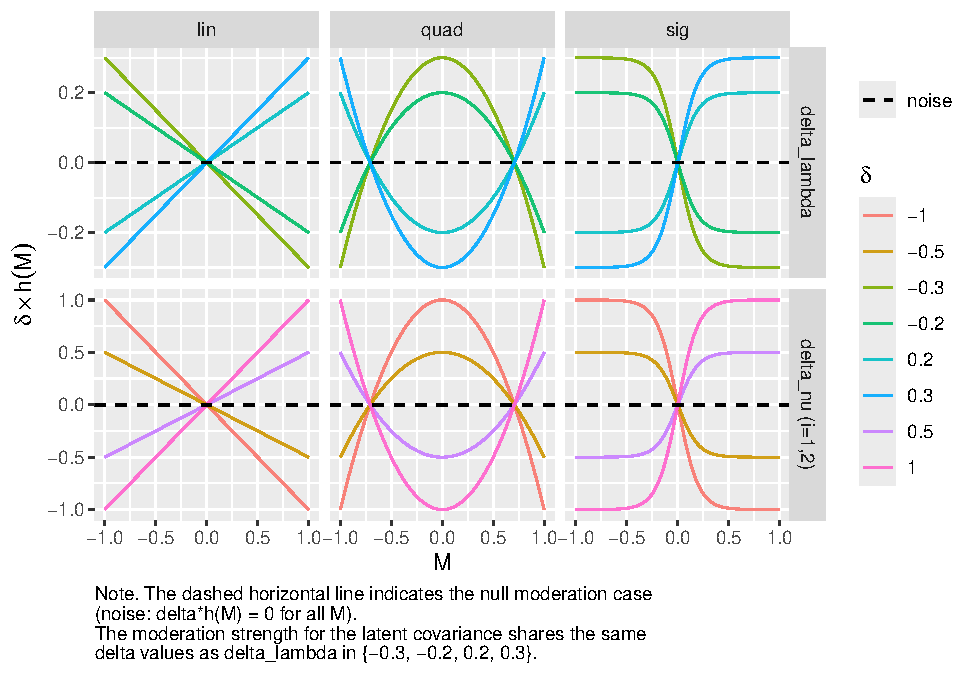
\includegraphics[keepaspectratio]{prereg_files/figure-latex/unnamed-chunk-1-1.pdf}}

\subsubsection{Factor Loadings}\label{factor-loadings}

The baseline factor loadings were fixed to a discrete value of
\(\lambda_{xi} = 0.7\).\\
Variation in loadings across simulation conditions arises exclusively
through the presence or absence of moderation, which is treated as a
fully crossed factor in the grid design.

\subsubsection{Moderated items}\label{moderated-items}

At the population level, the baseline (unmoderated) measurement model is
specified with a single latent factor and four indicators. The factor
loading matrix is constructed such that all four indicators share a
common loading value \(\lambda\):

\[
\boldsymbol{\Lambda}_x =
\begin{bmatrix}
\lambda_1 \\
\lambda_2 \\
\lambda_3 \\
\lambda_4
\end{bmatrix}
\]

The latent factor variance is fixed at a prespecified constant value
\(\psi_{\eta}= 1\) and is held constant across all simulation
conditions.

For each condition involving moderation, the loading of item \(i\) is
defined as a deterministic function of the moderator \(Z\):

\[
\lambda_{xi}(Z) = \lambda_{xi} + \delta_{\lambda} Z,
\quad Z \in [-1, 1].
\]

The parameter \(\delta_{\lambda}\) represents the strength of the
moderation effect and is specified using a discrete set of admissible
values chosen to ensure that the moderated loading remains within a
psychometrically plausible interval:

\[
\lambda_{xi}(Z) \in [0.3,\, 1.0].
\]

Given the fixed baseline loading \(\lambda_{xi}=0.7\), this constraint
yields an admissible range \[
\delta_{\lambda} \in [-0.4,\, 0.3].
\]

\(\delta_{\lambda}\) is evaluated at the following discrete levels:

\[
\delta_{\lambda} \in \{-0.3,\,-0.2,\,0.2,\,0.3\}.
\]

For moderator transformations beyond the linear case (quadratic or
sigmoid), the functional form of \(\lambda_{xi}(Z)\) is adapted
accordingly, and the same discrete set of admissible moderation
strengths is applied. This yields fully crossed combinations of (i) type
of moderator transformation, (ii) number of moderated items, and (iii)
moderation strength.

\subsubsection{Factor loading matrix}\label{factor-loading-matrix}

\[
\boldsymbol{\Lambda}_x(Z) =
\begin{bmatrix}
\lambda_1(Z) \\
\lambda_2(Z) \\
\lambda_3(Z)\\
\lambda_4(Z)
\end{bmatrix}
\]

Under partial moderation, only \(\lambda_1(Z)\) and \(\lambda_2(Z)\)
depend on \(Z\), while \(\lambda_3(Z)=\lambda_3\) and
\(\lambda_4(Z)=\lambda_4\). Under full moderation, all four loadings
vary with \(Z\).

\textbf{Null Model:} Neither factor loadings, nor intercepts are
moderated via Z. There is no moderation present in this DGP.

\textbf{Full moderation (Model 1.1):} All factor loadings and all
intercepts vary with \(Z\): \[
    \lambda_{xi}(Z) = \lambda_{xi} + \delta_{\lambda} Z, 
    \qquad
    \nu_{i}(Z) = \nu_{i} + \delta_{\nu} Z,
  \] \textbf{Partial moderation (Model 1.2):} Only the loadings of items
\(1\) and \(2\) and their intercepts can be moderated by Z: \[
    \lambda_{x1}(Z) = \lambda_{x1} + \delta_{\lambda} Z,
    \qquad
    \lambda_{x2}(Z) = \lambda_{x2} + \delta_{\lambda} Z,
  \] \[
    \nu_{x1}(Z) = \nu_{x1} + \delta_{\nu} Z,
    \nu_{x2}(Z) = \nu_{x2} + \delta_{\nu} Z,
  \] whereas all remaining loadings and intercepts as well as residual
variances \((\theta_{i0})\) remain fixed at their baseline values.

\subsubsection{Residual Variances}\label{residual-variances}

Item reliabilities are varied deterministically across simulation
conditions using the fixed grid. \[
Reliability_i \in \{0.60,\,0.70,\,0.80,\,0.95\}
\]

Baseline residual variances are derived analytically from a fixed latent
variance \(\psi_\eta=\psi_0>0\) and indicator-specific reliability
values: \[
Reliability_i=\frac{\lambda_{xi}^2 \psi_0}{\lambda_{xi}^2 \psi_0 + \theta_{i0}}\quad \Rightarrow \quad\theta_{i0}=\frac{\lambda_{xi}^2 \psi_0(1-\text{Reliability}_i)}
     {\text{Reliability}_i}.
\] \#\#\# Intercepts

Intercept moderation is manipulated via two fully crossed factors:\\
(i) the pattern of moderated items and\\
(ii) the magnitude of the moderation effect. For each indicator \(i\),
the intercept is modeled as \[
\nu_i(Z) = \nu_i + \delta_{\nu} Z,
\] where \(\nu_i\) denotes the baseline intercept and \(\delta_{\nu}\)
controls the strength and direction of intercept moderation. The pattern
of moderated items is varied across three levels:

\textbf{No intercept moderation:}

\(\delta_{\nu} = 0\) for all \(i = 1,\dots,4\), such that \[
  \nu_i(Z) = \nu_i \quad \text{for all } i.
\]

\textbf{Partial intercept moderation (items 1 and 2):}

\[
    \delta_{\nu} \in \{-1.0,\,-0.5,\,0.5,\,1.0\} \quad \text{for } i \in \{1,2\},
    \qquad
    \delta_{\nu} = 0 \quad \text{for } i \in \{3,4\},
\] such that only \(\nu_1(Z)\) and \(\nu_2(Z)\) vary with \(Z\).

\textbf{Full intercept moderation (all items):}

\[
    \delta_{\nu} \in \{-1.0,\,-0.5,\,0.5,\,1.0\} \quad \text{for } i = 1,\dots,4,
\] such that the intercepts of all four indicators vary with \(Z\).

Baseline intercepts are varied deterministically across simulation
conditions using the fixed grid \[
\nu_i \in \mathcal{G}_\nu = \{-1,\, 0,\, 1\},
  \] providing low, medium, and high intercept levels centered around
zero.

\subsubsection{Latent Distribution}\label{latent-distribution}

Latent mean moderation was specified deterministically as: \[
\mu_\eta(Z) = \alpha + \delta_\eta Z,
\]

with both parameters selected from discrete sets:

\[
\alpha \in \{0\}, \qquad
\delta_\eta \in \{-1.0,\,-0.5,\,0.5,\,1.0\}.
\]

The latent variance was modeled to be fixed at 1.

\pagebreak

\subsubsection{Analytical Model Study 1}\label{analytical-model-study-1}

\begin{center}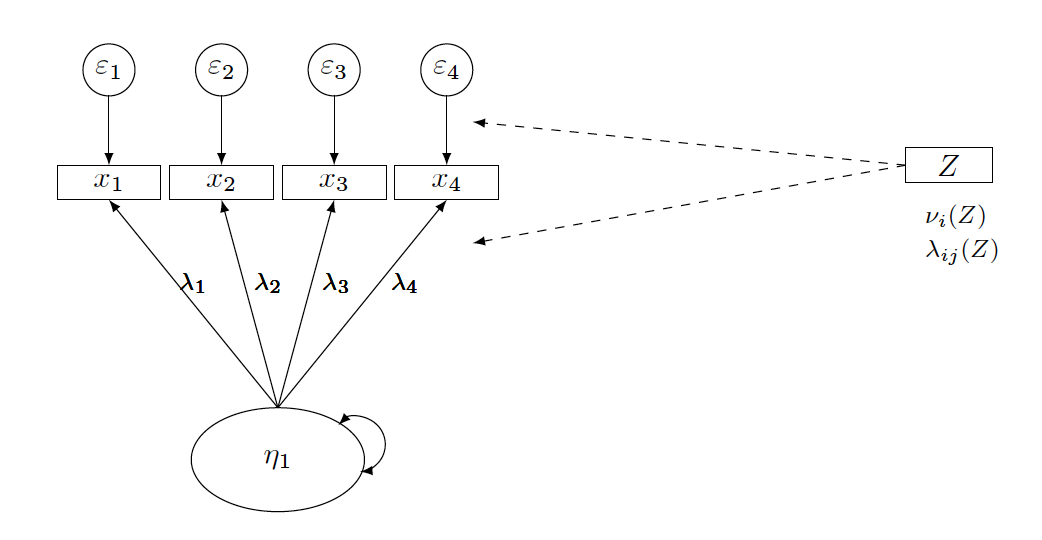
\includegraphics[width=0.7\linewidth]{presentation/tikz_model1} \end{center}

The analytical model will also have one latent factor \(\eta_1\). With
four manifest indicators \({x_1,..., x_4}\), their factor loadings
\({\lambda_1,..., \lambda_4}\) and their respective residuals
\({\epsilon_1,..., \epsilon_4}\). In the analytical model the residuals
will be assumed and modeled to be uncorrelated. Furthermore, the model
includes a moderator variable \(Z\), which can moderate the intercepts
and factor loadings from none, one or two of the manifest variables. The
moderator variable \(Z\) will be modeled as linear or quadratic.

\subsection{Study 2}\label{study-2}

\subsection{Two Factors with Moderator
Effects}\label{two-factors-with-moderator-effects}

We specify a confirmatory factor analysis model with two latent factors,
\(\eta_1\) and \(\eta_2\), and seven observed indicators
\(\mathbf{x} = (x_1, \dots, x_4)^\top\) and
\(\mathbf{y} = (y_1, \dots, y_3)^\top\). Along their respective
residuals \({\epsilon_1,...,\epsilon_4}\) and
\({\delta_1,..., \delta_3}\). The first factor loads onto indicators
\(x_1\) to \(x_4\), the second onto \(y_1\) to \(y_3\). A continuous
moderator variable \(Z\) introduces conditional heterogeneity into
selected measurement parameters (i.e.~intercepts, loadings and latent
factor covariance) using one of three functional forms (linear,
quadratic or sigmoid).

\[
\mathbf{x} = \boldsymbol{\nu}_x(Z) + \boldsymbol{\Lambda}_x(Z)\,\eta_1 + \boldsymbol{\varepsilon}(Z),
\] \[
\mathbf{y} = \boldsymbol{\nu}_y(Z) + \boldsymbol{\Lambda}_y(Z)\,\eta_2 + \boldsymbol{\delta}(Z),
\]

where:

\begin{itemize}
\tightlist
\item
  \(\boldsymbol{\nu}_x(Z)\) and \(\boldsymbol{\nu}_y(Z)\) are the
  \(4 \times 1\) and \(3 \times 1\) vectors of intercepts for
  \(\mathbf{x}\) and \(\mathbf{y}\), respectively,
\item
  \(\boldsymbol{\Lambda}_x(Z)\) is the \(4 \times 1\) loading vector for
  \(\eta_1\), and \(\boldsymbol{\Lambda}_y(Z)\) is the \(3 \times 1\)
  loading vector for \(\eta_2\),
\item
  \(\boldsymbol{\varepsilon}(Z) \sim \mathcal{N}\bigl(\mathbf{0}, \boldsymbol{\Theta}_x(Z)\bigr)\)
  and
  \(\boldsymbol{\delta}(Z) \sim \mathcal{N}\bigl(\mathbf{0}, \boldsymbol{\Theta}_y(Z)\bigr)\)
  are the residual vectors for \(\mathbf{x}\) and \(\mathbf{y}\),
\item
  \(\boldsymbol{\eta} = (\eta_1, \eta_2)^\top \sim \mathcal{N}\bigl(\boldsymbol{\mu}_\eta(Z), \boldsymbol{\Phi}_\eta(Z)\bigr)\)
  is the latent factor vector,
\item
  \(Z = h(M)\) is the effective moderator entering the model equations,
  obtained by transforming a raw continuous covariate \(M\).
\end{itemize}

\subsubsection{Moderator
Transformation}\label{moderator-transformation-1}

Let \(M \sim \mathcal{U}(-1,1)\) denote a bounded continuous covariate.

The effective moderator is defined as \[
Z = h(M),
\]

where \[h(\cdot)\] is chosen from the following deterministic
transformation functions. Each transformation type is treated as a
distinct condition in the simulation design:

\begin{enumerate}
\def\labelenumi{\arabic{enumi}.}
\item
  \textbf{Linear:} \[
  h(M) = M
  \] In this case, the effective moderator is bounded to the interval
  \((-1,1)\) and symmetric around zero.
\item
  \textbf{Sigmoid:} \[
  h(M) = a + \frac{b-a}{1 + \exp\!\bigl(-k(M-c)\bigr)},
  \qquad a=-1,\; b=1,\; c=0,\; k>0.
  \] This transformation maps the input to the open interval \((-1, 1)\)
  and yields a bounded moderator symmetric around zero, exhibiting
  diminishing sensitivity at extreme values.
\item
  \textbf{Quadratic:} \[
  h(M) = 2M^2 - 1
  \] This transformation captures symmetric nonlinear moderation as a
  function of distance from the center while remaining bounded in
  \((-1,1)\).
\item
  \textbf{Noise:} \[
  h(M) = 0
  \]
\end{enumerate}

In this condition, the moderator has no effect on any model parameter
and serves as a non-informative (noise) moderator.

Null moderation is represented by the noise-moderator condition
\((Z=0)\), not by \(\delta=0\); moderation coefficients are held fixed
across conditions. All parameter-level moderation effects are specified
as linear functions of the effective moderator \(Z\). Nonlinearity in
moderation arises exclusively through the transformation \(Z = h(M)\),
not through nonlinear parameter functions.

\subsubsection{Factor Loadings}\label{factor-loadings-1}

For each latent factor, all baseline loadings for that factor are fixed
at 0.7. For the two-factor model in Study\textasciitilde2, this yields

\[
\boldsymbol{\Lambda}_x =
\begin{bmatrix}
0.7\\
0.7\\
0.7\\
0.7
\end{bmatrix},
\qquad
\boldsymbol{\Lambda}_y =
\begin{bmatrix}
0.7\\
0.7\\
0.7
\end{bmatrix},
\]

Moderation of factor loadings is introduced only for the first two
\(x\)-indicators. For each moderated indicator \(i \in \{1,2\}\), \[
\lambda_{xi}(Z) = \lambda_{xi} + \delta_{\lambda} Z .
\]

To ensure that moderated loadings remain within an admissible interval,
\[
\lambda_{xi}(Z) \in [0.3,\,1.0],
\]

the moderation coefficients are restricted to \[
\delta_{\lambda} \in [-0.4,\,0.3],
\]

and evaluated on the discrete grid (leaving out the zero effect) \[
\delta_{\lambda} \in \{-0.3,\,-0.2,\,0.2,\,0.3\}.
\]

Thus, the loading matrices take the form \[
\boldsymbol{\Lambda}_x(Z)=
\begin{bmatrix}
\lambda_{x1}(Z)\\
\lambda_{x2}(Z)\\
0.7\\
0.7
\end{bmatrix},
\qquad
\boldsymbol{\Lambda}_y(Z)=
\begin{bmatrix}
0.7\\
0.7\\
0.7
\end{bmatrix},
\]

yielding fully crossed combinations of (i) moderator transformation type
\(Z=h(M)\), (ii) moderated vs.~unmoderated indicators, and (iii)
moderation strength \(\delta_{\lambda}\).

\subsubsection{Residual Variances}\label{residual-variances-1}

Item reliabilities are varied deterministically across simulation
conditions using the fixed grid. \[
Reliability_i \in \{0.60,\,0.70,\,0.80,\,0.95\}
\]

Baseline residual variances are derived analytically from a fixed latent
variance \(\psi_\eta=\psi_0>0\) and indicator-specific reliability
values:

\[
Reliability_i=\frac{\lambda_{xi}^2 \psi_0}{\lambda_{xi}^2 \psi_0 + \theta_{i0}}\quad \Rightarrow \quad\theta_{i0}=\frac{\lambda_{xi}^2 \psi_0(1-\text{Reliability}_i)}
     {\text{Reliability}_i}.
\] \#\#\# Intercepts

Intercept moderation is manipulated via two fully crossed factors:\\
(i) the pattern of moderated items and\\
(ii) the magnitude of the moderation effect. For each indicator \(i\),
the intercept is modeled as \[
\nu_i(Z) = \nu_i + \delta_{\nu} Z,
\] where \(\nu_i\) denotes the baseline intercept and \(\delta_{\nu}\)
controls the strength and direction of intercept moderation. The pattern
of moderated items is varied across three levels:

\textbf{No intercept moderation:} \(\delta_{\nu} = 0\) for all
\(i = 1,\dots,4\), such that \[
  \nu_i(Z) = \nu_i \quad \text{for all } i.
  \]

\textbf{Partial intercept moderation (items 1 and 2):}\\
\[
    \delta_{\nu} \in \{-1.0,\,-0.5,\,0.5,\,1.0\} \quad \text{for } i \in \{1,2\},
    \qquad
    \delta_{\nu} = 0 \quad \text{for } i \in \{3,4\},
    \] such that only \(\nu_1(Z)\) and \(\nu_2(Z)\) vary with \(Z\).

\textbf{Full intercept moderation (all items):}\\
\[
    \delta_{\nu} \in \{-1.0,\,-0.5,\,0.5,\,1.0\} \quad \text{for } i = 1,\dots,4,
  \] such that the intercepts of all four indicators vary with \(Z\).
Baseline intercepts are set to 1.

\subsubsection{Latent Variable
Distribution}\label{latent-variable-distribution}

Latent means are held constant at zero for both latent factors:

\[
\boldsymbol{\mu}_\eta(Z) = 
\begin{bmatrix}
0 \\[4pt]
0
\end{bmatrix}.
\]

Latent variances are allowed to vary with the effective moderator \(Z\)
through the log-linear specification

\[
\sigma^2_{\eta_j}(Z)
  = \exp\!\left(\beta_{0j} + \beta_{1j} Z\right),
\qquad j = 1,2,
\] ensuring positivity for all variance values.

The baseline variance is set to 1 and moderation strength is selected
from a discrete grid:

\[
\delta_{\sigma_\eta} \in \{-0.3,\,-0.2,\,0.2,\,0.3\}.
\]

The latent covariance between \(\eta_1\) and \(\eta_2\) is fixed across
all conditions:

\[
\phi_{12}(Z) = 0.4,
\]

yielding the latent covariance matrix \[
\boldsymbol{\Phi}_\eta(Z)
=
\begin{bmatrix}
\sigma^2_{\eta_1}(Z) & 0.4 \\
0.4 & \sigma^2_{\eta_2}(Z)
\end{bmatrix}.
\]

\begin{sidewaysfigure}
\noindent{\textbf{Analytical Models Study 2}}
\vspace{\baselineskip}
\vspace{\baselineskip}
\centering

\begin{subfigure}[b]{0.47\textwidth}
    \centering
    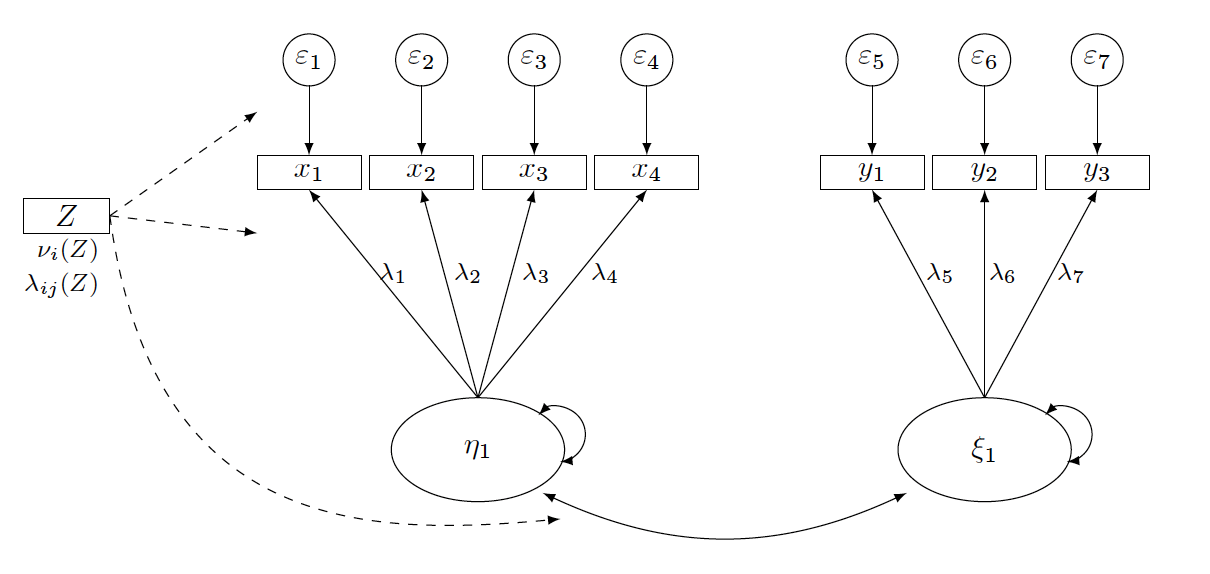
\includegraphics[width=\linewidth]{presentation/tikz_model2.0.png}
    \caption{Model 2.0}
\end{subfigure}
\hspace{0.3cm} % tighter space
\begin{subfigure}[b]{0.47\textwidth}
    \centering
    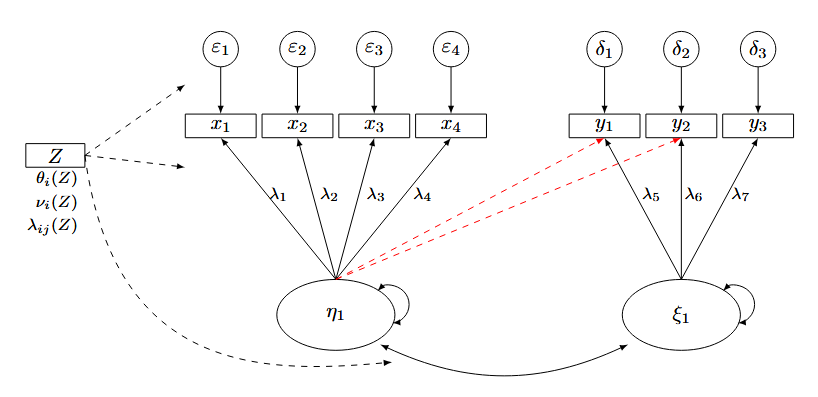
\includegraphics[width=\linewidth]{presentation/tikz_model2.1.png}
    \caption{Model 2.1}
\end{subfigure}

\caption{We specify a confirmatory factor analysis model with two latent factors, $\eta_1$ and $\xi_1$, and seven observed indicators, $\mathbf{x} = (x_1, \dots, x_4)^\top$ and $\mathbf{y} = (y_1, y_2, y_3)^\top$, along with their respective residuals, $\varepsilon_1, \dots, \varepsilon_4$ and $\delta_1, \delta_2, \delta_3$. The first factor, $\eta_1$, loads onto indicators $x_1$ to $x_4$, while the second factor, $\xi_1$, loads onto indicators $y_1$ to $y_3$. A continuous moderator variable $Z$ introduces conditional heterogeneity into selected measurement parameters, including intercepts, factor loadings, and latent factor covariance, using one of two functional forms (linear or quadratic). Red dashed arrows indicate model misspecifications.}
\end{sidewaysfigure}

\pagebreak

\subsection{What will be the different factors of the data-generating
mechanism?}\label{what-will-be-the-different-factors-of-the-data-generating-mechanism}

The simulation design includes several manipulated factors that govern
the data-generating mechanism (DGM). These factors are varied across
simulation conditions and apply consistently to both studies, unless
otherwise noted.

\subsubsection{Core DGM Factors (Applied in Both
Studies)}\label{core-dgm-factors-applied-in-both-studies}

The following factors are systematically varied in both studies using a
grid search design:

\paragraph{Functional form of
moderation}\label{functional-form-of-moderation}

The moderator variable \(Z\) is defined as a transformation of
\(X \in [-1, 1]\), evaluated systematically using three functional
forms: 1. Linear 2. Quadratic 3. Sigmoid

\paragraph{Strength of moderation}\label{strength-of-moderation}

In each case where parameters are subjected to moderation, the strength
of the moderation \(\delta\) is varied:

\(\delta_{\lambda}\) is evaluated at the following discrete levels:

\[
\delta_{\lambda} \in \{-0.3,\,-0.2,\,0.2,\,0.3\}.
\]

\[
\delta_{\nu} \in \{-1.0,\,-0.5,\,0.5,\,1.0\} \quad \text{for } i \in \{1,2\},
    \qquad
    \delta_{\nu} = 0 \quad \text{for } i \in \{3,4\},
\]

\paragraph{Model misspecification of moderator
form}\label{model-misspecification-of-moderator-form}

The DGM defines \(Z\) using one of the three functional forms above,
while the analytical model assumes either a \emph{linear} or
\emph{quadratic} moderator effect.

\subsubsection{Study-Specific Factors}\label{study-specific-factors}

\paragraph{Study 1.}\label{study-1.}

Focuses on functional form misspecification and data-related conditions:

\textbf{Sample sizes:} \(N \in \{300, 500, 700, 1000\}\)
\textbf{Intercepts:} Intercept baselines are varied across simulation
conditions \(\nu_i \in \mathcal{G}_\nu = \{-1,\, 0,\, 1\}\)\\
\textbf{Indicator reliabilities:} \emph{Low} (.6), \emph{moderate} (.7),
\emph{moderate to high} (.8), or \emph{high} (.95).

\paragraph{Study 2.}\label{study-2.}

Builds on Study 1 and introduces additional model misspecification in
the factor structure:

\textbf{Structural model misspecifications:} (between-subjects factor)
\textbf{1. No misspecification:} Factor structure matches the analysis
model. \textbf{2. Cross-loadings:} Items \(y_5\), \(y_6\) additionally
load on a second latent factor:\\
\textbf{Latent Covariance:} The latent covariance is moderated by \(Z\).
The baseline variance is set to 1 and moderation strength is selected
from:

\[
\delta_{\sigma_\eta} \in \{-0.3,\,-0.2,\,0.2,\,0.3\}.
\]

\subsubsection{If there is more than one factor: How will the factor
levels be combined and how many simulation conditions will this
create?}\label{if-there-is-more-than-one-factor-how-will-the-factor-levels-be-combined-and-how-many-simulation-conditions-will-this-create}

We employ a full grid search, in which parameter values are sampled from
pre-specified discrete values. A total of 6000 simulation replications
should ideally be conducted. This number was chosen to ensure that the
confidence intervals for key estimated proportions (e.g., power or Type
I error rates near \(p = 0.8\) achieve an approximate width of
\(\pm 1\%\). This is based on the calculation:

\[
\text{SE} = 2 \times \sqrt{\frac{p(1-p)}{6000}},
\] which yields a standard error consistent with the desired precision
for evaluating simulation outcomes within this study. To ensure
computational feasibility, we propose an iterative approach whereby
initial pilot simulations \(n=100\) are conducted to amongst others,
estimate the needed simulation time. These estimates then inform a more
principled determination of the total number of replications, targeting
a predefined precision threshold.

The factors that vary across simulation conditions include:

\begin{itemize}
\tightlist
\item
  The functional form of moderator effects (linear, quadratic, sigmoid)
\item
  The type of moderated parameters (e.g., factor loadings, intercepts)
\item
  The degree of model misspecification (none, cross-loadings, correlated
  residuals, combined)
\item
  Item reliabilities (ranging from 0.6 to 0.95)
\item
  Moderator strength parameters
\item
  Sample sizes per group (i.e.~300, 500, 700, 1000)
\end{itemize}

\subsection{Estimands and Targets}\label{estimands-and-targets}

\subsubsection{What will be the estimands and/or targets of the
simulation
study?}\label{what-will-be-the-estimands-andor-targets-of-the-simulation-study}

The primary estimands in this simulation study pertain to the detection
and accurate estimation of measurement non-invariance (MI) due to
moderation effects on measurement parameters. Specifically, we assess
whether the estimation methods compared can correctly identify the
presence or absence of moderation in factor loadings, intercepts, and
residual variances, reflecting the true data-generating structure.
Consequently, key simulation outcomes include Type I error rates and
statistical power associated with detecting such moderation effects, as
well as bias and variability in the recovered parameter estimates.

Secondary estimands include model-level indicators of fit (e.g., RMSEA
with confidence intervals, SRMR, CFI), which serve as auxiliary
diagnostics for methods that yield such metrics (i.e., MNLFA). These are
not applicable to tree-based approaches and are thus interpreted as
method-specific targets rather than general evaluative criteria.

\subsection{Methods}\label{methods}

\subsubsection{How many and which methods will be included and which
quantities will be
extracted?}\label{how-many-and-which-methods-will-be-included-and-which-quantities-will-be-extracted}

We will compare the following methods:

\begin{enumerate}
\def\labelenumi{\arabic{enumi})}
\item
  \textbf{Moderated Nonlinear Factor Analysis:} MNLFA was initially
  introduced by Bauer and Hussong (2009) within the framework of
  integrative data analysis and was subsequently extended into a general
  approach for assessing measurement invariance and moderation (Bauer
  2017). The fundamental principle of MNLFA is the parameterization of
  both measurement and structural model parameters as functions of one
  or more moderator variables. MNLFA accommodates both frequentist
  estimation methods, such as maximum likelihood (ML), and Bayesian
  techniques, including Markov Chain Monte Carlo (MCMC), thereby
  offering methodological flexibility aligned with specific analytical
  objectives (Münch and Koch 2024).
\item
  \textbf{SEM Trees:} Structural equation modeling (SEM) trees were
  originally introduced by Brandmaier et al. (2013) as a way to
  systematically search for important covariates and their interactions
  in data, creating homogeneous subgroups. The method was refined later
  on by Brandmaier et al. (2016) and Arnold, Voelkle, and Brandmaier
  (2021). SEM trees and forests are data-driven, non-parametric methods
  that build upon the decision tree paradigm, thus using recursive
  partitioning to identify latent subgroups in which model parameters
  differ, without assuming specific functional forms or predefined
  covariate effects. These approaches allow for nonlinear moderation of
  factor loadings and can reveal complex interaction effects, enabling
  the exploratory detection of DIF.
\end{enumerate}

For the parametric MNLFA, we will extract estimated moderated parameters
(e.g., factor loadings, intercepts), their associated standard errors,
and two-sided \(p\)-values for testing the null hypothesis of no
moderation effect. Additionally, model fit indices such as RMSEA (with
confidence intervals), SRMR, and CFI will be recorded.

For the parameter estimates and fit indices, we will summarize their
distributions across simulation replications by reporting key quantiles
(2.5th, 50th, and 97.5th percentiles). The null hypothesis will be
rejected if the associated \(p\)-value is less than the conventional
significance level of 0.05.

In contrast, non-parametric Tree-based approaches do not yield direct
parameter estimates with standard errors. We use score-based
SEM-trees(Arnold, Voelkle, and Brandmaier 2021). Their detection of MI/
non-invariance is operationalized via the presence of at least one split
in the correct condition at the correct respective level of focus
parameters. Those splits, introducing a subgroup, will be evaluated at
the significance level: 0.05, using the ``maximally selected
likelihood-ratio''(Arnold, Voelkle, and Brandmaier 2021). Additionally,
a Bonferroni-Holm correction to account for multiple comparisons at each
node. The trees will be allowed to split on the focus parameters
relevant for the invariance testing (the means of the intercepts, factor
loadings and the latent covariance in study 2). Candidate subgroup
structures are assessed by testing whether they produce statistically
significant differences in the specified model parameters across groups.
Differences in factor variances between subgroups are permitted in the
model, but they are not used as criteria for selecting or evaluating
covariates. Furthermore, pre-pruning will be applied, limiting the
maximum depth of the tree to 1 and \texttt{min.N} and
\texttt{min.bucket} are set to be equal and both set to XX?. Because the
MNLFA also considers directly the form of the moderation, which the SEM
trees do not, we further want to use SEM forests for generating partial
dependence plots to get an approximation of the functional form of the
moderating variables.\\
With this distinction we aim to ensure that each method is evaluated
according to its own inferential framework, while maintaining
comparability in terms of its ability to detect MI reliably.

\subsection{Performance Measures}\label{performance-measures}

\subsubsection{Which performance measures will be
used?}\label{which-performance-measures-will-be-used}

For the MNLFA \textbf{exclusively}, we will evaluate the following
performance measures:

\textbf{Bias:} The average difference between the estimated parameter
\(\hat{\theta}\) and the true parameter \(\theta\), defined as \[
\widehat{\text{Bias}} = \frac{1}{n_{\text{sim}}} \sum_{i=1}^{n_{\text{sim}}} \hat{\theta}_i - \theta,
\] where \(n_{\text{sim}}\) is the number of simulation replications.

\textbf{Absolute Bias:} \[
\widehat{\text{AbsBias}} = \frac{1}{n_{\text{sim}}} \sum_{i=1}^{n_{\text{sim}}} \left| \hat{\theta}_i - \theta \right|.
\]

\textbf{Relative Bias:} (expressed as a proportion of the true
parameter) \[
\widehat{\text{RelBias}} = \frac{\widehat{\text{Bias}}}{|\theta|} \quad \text{for } \theta \neq 0.
\]

\textbf{Root Mean Squared Error (RMSE):} \[
\widehat{\text{RMSE}} = \sqrt{ \frac{1}{n_{\text{sim}}} \sum_{i=1}^{n_{\text{sim}}} (\hat{\theta}_i - \theta)^2}.
\]

\textbf{Coverage Probability:} The proportion of confidence intervals
that contain the true parameter \(\theta\).

\textbf{Model Fit Indices:} (e.g., RMSEA) will be reported if
applicable, computed according to their standard definitions.

For the SEM trees \textbf{as well as} for the MNLFA we will evaluate:

\textbf{Type I Error Rate and Power:} The rejection rate of the null
hypothesis at significance level \(\alpha = 0.05\), calculated as \[
\widehat{\text{RRate}} = \frac{1}{n_{\text{sim}}} \sum_{i=1}^{n_{\text{sim}}} \mathbf{1}(p_i \leq 0.05),
\] where \(\mathbf{1}(\cdot)\) is the indicator function.

Performance measures calculated for multiple parameters (e.g., factor
loadings) will be aggregated by reporting the mean value across
parameters.

\subsubsection{How will Monte Carlo uncertainty of the estimated
performance measures be calculated and
reported?}\label{how-will-monte-carlo-uncertainty-of-the-estimated-performance-measures-be-calculated-and-reported}

We will quantify Monte Carlo uncertainty using Monte Carlo Standard
Errors (MCSEs) for each performance measure, calculated as follows:

The \textbf{Rejection Rate} refers to the proportion of simulated
datasets in which a null hypothesis is rejected, commonly used to
estimate empirical Type I error rates or statistical power. The
\textbf{MCSE for the Rejection Rate} is calculated assuming a binomial
distribution of rejections across \(n_{\text{sim}}\) simulation
replications, which reflects the standard error of a proportion
estimator:

\[
\text{MCSE}_{\widehat{\text{RRate}}} = \sqrt{\frac{\widehat{\text{RRate}} (1 - \widehat{\text{RRate}})}{n_{\text{sim}}}},
\]

For \textbf{Bias}, MCSE is calculated based on the sample variance of
the specific parameter estimates across simulation replications:

\[
\text{MCSE}_{\widehat{\text{Bias}}} = \frac{S_{\hat{\theta}}}{\sqrt{n_{\text{sim}}}},
\]

where \[
S_{\hat{\theta}} = \sqrt{\sum_{i=1}^{n_{\text{sim}}}{ \{\hat{\theta}_i - (\sum_{i=1}^{n_{\text{sim}}}\hat{\theta}_i/n_{\text{sim}})\}^2}/(n_{\text{sim}} - 1)}
\] is the sample standard deviation of the effect estimates.

Siepe et al. (2024) ,Morris, White, and Crowther (2019) and Whitehead
(1993)

\subsection{How many simulation repetitions will be used for each
condition?}\label{how-many-simulation-repetitions-will-be-used-for-each-condition}

A total of 6000 simulation replications should ideally be conducted.
This number was chosen to ensure that the confidence intervals for key
estimated proportions (e.g., power or Type I error rates near
\(p = 0.8\)) achieve an approximate width of \(\pm 1\%\). This is based
on the calculation: \[
\text{SE} = 2 \times \sqrt{\frac{p(1-p)}{6000}},
\] which yields a standard error consistent with the desired precision
for evaluating simulation outcomes within this study. To ensure
computational feasability, we propose an iterative approach whereby
initial pilot simulations \(n=100\) are conducted to amongst others,
estimate the needed simulation time. These estimates then inform a more
principled determination of the total number of replications, targeting
a predefined precision threshold.

\subsection{How will missing values due to non-convergence or other
reasons be
handled?}\label{how-will-missing-values-due-to-non-convergence-or-other-reasons-be-handled}

Non-convergence or other missing values may occur during model
estimation. We plan to:

\begin{itemize}
\tightlist
\item
  Exclude only the specific simulation replicates that fail to converge
  for a given method while retaining data from other methods within the
  same replication.
\item
  Report the proportion of non-converged cases per method and condition.
\item
  If the proportion of non-convergence exceeds a pre-specified threshold
  (e.g., 5\%), we will flag the corresponding simulation condition and
  interpret results with caution.
\end{itemize}

No imputation of missing estimates will be performed.

\subsection{How do you plan on interpreting the performance
measures?}\label{how-do-you-plan-on-interpreting-the-performance-measures}

\emph{Answer:}

\section{Other}\label{other}

\subsection{Which statistical software/packages do you plan to
use?}\label{which-statistical-softwarepackages-do-you-plan-to-use}

\emph{Answer:}

\subsection{Which computational environment do you plan to
use?}\label{which-computational-environment-do-you-plan-to-use}

The simulation study will be conducted in R (R Core Team 2025).

\subsection{Which other steps will you undertake to make simulation
results
reproducible?}\label{which-other-steps-will-you-undertake-to-make-simulation-results-reproducible}

We are planning to make the code of this project publicly available.
Software and packages will be documented via ``renv''(Ushey and Wickham
2026) and Docker. Furthermore, we are planning to use the ``repro''
package, as well as the ``reproducibleRchunks'' package for better
reproducibility.

\pagebreak

\subsection*{References}\label{references}
\addcontentsline{toc}{subsection}{References}

\phantomsection\label{refs}
\begin{CSLReferences}{1}{0}
\bibitem[\citeproctext]{ref-Arnold2021}
Arnold, M., M. C. Voelkle, and A. M. Brandmaier. 2021. {``Score-Guided
Structural Equation Model Trees.''} \emph{Frontiers in Psychology} 11:
3913. \url{https://doi.org/10.3389/fpsyg.2020.564403}.

\bibitem[\citeproctext]{ref-Bauer2017}
Bauer, D. J. 2017. {``A More General Model for Testing Measurement
Invariance and Differential Item Functioning.''} \emph{Psychological
Methods} 22 (3): 507--26. \url{https://doi.org/10.1037/met0000077}.

\bibitem[\citeproctext]{ref-Bauer2020}
Bauer, D. J., W. C. M. Belzak, and V. T. Cole. 2020. {``Simplifying the
Assessment of Measurement Invariance over Multiple Background Variables:
Using Regularized Moderated Nonlinear Factor Analysis to Detect
Differential Item Functioning.''} \emph{Structural Equation Modeling: A
Multidisciplinary Journal} 27 (1): 43--55.
\url{https://doi.org/10.1080/10705511.2019.1642754}.

\bibitem[\citeproctext]{ref-Bauer2009}
Bauer, D. J., and A. M. Hussong. 2009. {``Psychometric Approaches for
Developing Commensurate Measures Across Independent Studies: Traditional
and New Models.''} \emph{Psychological Methods} 14 (2): 101--25.
\url{https://doi.org/10.1037/a0015583}.

\bibitem[\citeproctext]{ref-Brandmaier2013}
Brandmaier, A. M., T. von Oertzen, J. J. McArdle, and U. Lindenberger.
2013. {``Structural Equation Model Trees.''} \emph{Psychological
Methods} 18 (1): 71--86. \url{https://doi.org/10.1037/a0030001}.

\bibitem[\citeproctext]{ref-Brandmaier2016}
Brandmaier, A. M., J. J. Prindle, J. J. McArdle, and U. Lindenberger.
2016. {``Theory-Guided Exploration with Structural Equation Model
Forests.''} \emph{Psychological Methods} 21 (4): 566--82.
\url{https://doi.org/10.1037/met0000090}.

\bibitem[\citeproctext]{ref-Buchberger2024}
Buchberger, E. S., C. T. Ngo, A. Peikert, A. M. Brandmaier, and M.
Werkle-Bergner. 2024. {``Estimating Statistical Power for Structural
Equation Models in Developmental Cognitive Science: A Tutorial in r.''}
\emph{Behavior Research Methods} 56 (7): 6862--79.
\url{https://doi.org/10.3758/s13428-024-02396-2}.

\bibitem[\citeproctext]{ref-SilvaDuxedaz2025}
Díaz, John Alexander Silva, Moritz Heene, and Andreas M. Brandmaier and.
2025. {``Evaluation of Structural Equation Model Forests' Performance to
Identify Omitted Influential Covariates.''} \emph{Structural Equation
Modeling: A Multidisciplinary Journal} 32 (2): 319--31.
\url{https://doi.org/10.1080/10705511.2024.2417866}.

\bibitem[\citeproctext]{ref-Kolbe2024}
Kolbe, Laura, Dylan Molenaar, Suzanne Jak, and Terrence D. Jorgensen.
2024. {``{Assessing Measurement Invariance with Moderated Nonlinear
Factor Analysis Using the R Package OpenMx}.''} \emph{Psychological
Methods} 29 (2): 388--406. \url{https://doi.org/10.1037/met0000501}.

\bibitem[\citeproctext]{ref-Lee2024}
Lee, S., S. Han, and S. W. Choi. 2024. {``A Bayesian Moderated Nonlinear
Factor Analysis Approach for DIF Detection Under Violation of the Equal
Variance Assumption.''} \emph{Journal of Educational Measurement} 61:
303--24. \url{https://doi.org/10.1111/jedm.12388}.

\bibitem[\citeproctext]{ref-Morris2019}
Morris, Tim P., Ian R. White, and Michael J. Crowther. 2019. {``Using
Simulation Studies to Evaluate Statistical Methods.''} \emph{Statistics
in Medicine} 38 (11): 2074--2102.
\url{https://doi.org/10.1002/sim.8086}.

\bibitem[\citeproctext]{ref-Muench2024}
Münch, F. F., and T. Koch. 2024. {``Testing Measurement and Structural
Invariance in Latent Mediation Models -- a Comparison of IPCR and
Bayesian MNLFA.''} Preprint.
\url{https://doi.org/10.31234/osf.io/zpgtn}.

\bibitem[\citeproctext]{ref-Rteam2025}
R Core Team. 2025. \emph{R: A Language and Environment for Statistical
Computing}. Vienna, Austria: R Foundation for Statistical Computing.
\url{https://www.R-project.org/}.

\bibitem[\citeproctext]{ref-Siepe2024}
Siepe, Björn S., František Bartoš, Tim P. Morris, Anne-Laure Boulesteix,
Daniel W. Heck, and Samuel Pawel. 2024. {``Simulation Studies for
Methodological Research in Psychology: A Standardized Structure for
Planning, Preregistration, and Reporting.''} \emph{Psychological
Methods}. \url{https://doi.org/10.1037/met0000695}.

\bibitem[\citeproctext]{ref-renv2026}
Ushey, Kevin, and Hadley Wickham. 2026. \emph{Renv: Project
Environments}. \url{https://doi.org/10.32614/CRAN.package.renv}.

\bibitem[\citeproctext]{ref-Whitehead1993}
Whitehead, John. 1993. {``{Sample Size Calculations for Ordered
Categorical Data}.''} \emph{Statistics in Medicine} 12 (24): 2257--71.
\url{https://doi.org/10.1002/sim.4780122404}.

\end{CSLReferences}

\end{document}
